% Options for packages loaded elsewhere
\PassOptionsToPackage{unicode}{hyperref}
\PassOptionsToPackage{hyphens}{url}
%
\documentclass[
  11pt,
]{article}
\usepackage{amsmath,amssymb}
\usepackage{lmodern}
\usepackage{ifxetex,ifluatex}
\ifnum 0\ifxetex 1\fi\ifluatex 1\fi=0 % if pdftex
  \usepackage[T1]{fontenc}
  \usepackage[utf8]{inputenc}
  \usepackage{textcomp} % provide euro and other symbols
\else % if luatex or xetex
  \usepackage{unicode-math}
  \defaultfontfeatures{Scale=MatchLowercase}
  \defaultfontfeatures[\rmfamily]{Ligatures=TeX,Scale=1}
\fi
% Use upquote if available, for straight quotes in verbatim environments
\IfFileExists{upquote.sty}{\usepackage{upquote}}{}
\IfFileExists{microtype.sty}{% use microtype if available
  \usepackage[]{microtype}
  \UseMicrotypeSet[protrusion]{basicmath} % disable protrusion for tt fonts
}{}
\makeatletter
\@ifundefined{KOMAClassName}{% if non-KOMA class
  \IfFileExists{parskip.sty}{%
    \usepackage{parskip}
  }{% else
    \setlength{\parindent}{0pt}
    \setlength{\parskip}{6pt plus 2pt minus 1pt}}
}{% if KOMA class
  \KOMAoptions{parskip=half}}
\makeatother
\usepackage{xcolor}
\IfFileExists{xurl.sty}{\usepackage{xurl}}{} % add URL line breaks if available
\IfFileExists{bookmark.sty}{\usepackage{bookmark}}{\usepackage{hyperref}}
\hypersetup{
  pdfauthor={Names},
  hidelinks,
  pdfcreator={LaTeX via pandoc}}
\urlstyle{same} % disable monospaced font for URLs
\usepackage[margin=1in]{geometry}
\usepackage{longtable,booktabs,array}
\usepackage{calc} % for calculating minipage widths
% Correct order of tables after \paragraph or \subparagraph
\usepackage{etoolbox}
\makeatletter
\patchcmd\longtable{\par}{\if@noskipsec\mbox{}\fi\par}{}{}
\makeatother
% Allow footnotes in longtable head/foot
\IfFileExists{footnotehyper.sty}{\usepackage{footnotehyper}}{\usepackage{footnote}}
\makesavenoteenv{longtable}
\usepackage{graphicx}
\makeatletter
\def\maxwidth{\ifdim\Gin@nat@width>\linewidth\linewidth\else\Gin@nat@width\fi}
\def\maxheight{\ifdim\Gin@nat@height>\textheight\textheight\else\Gin@nat@height\fi}
\makeatother
% Scale images if necessary, so that they will not overflow the page
% margins by default, and it is still possible to overwrite the defaults
% using explicit options in \includegraphics[width, height, ...]{}
\setkeys{Gin}{width=\maxwidth,height=\maxheight,keepaspectratio}
% Set default figure placement to htbp
\makeatletter
\def\fps@figure{htbp}
\makeatother
\setlength{\emergencystretch}{3em} % prevent overfull lines
\providecommand{\tightlist}{%
  \setlength{\itemsep}{0pt}\setlength{\parskip}{0pt}}
\setcounter{secnumdepth}{5}
\ifluatex
  \usepackage{selnolig}  % disable illegal ligatures
\fi

\title{\textbf{Title}}
\author{Names}
\date{\today}

\begin{document}
\maketitle
\begin{abstract}
This manuscript\ldots{} The main results are\ldots{}
\end{abstract}

\hypertarget{introduction}{%
\section{Introduction}\label{introduction}}

\hypertarget{data-and-methods}{%
\section{Data and Methods}\label{data-and-methods}}

\hypertarget{results}{%
\section{Results}\label{results}}

\hypertarget{simulations-uniform-ranks}{%
\subsection{Simulations: Uniform
Ranks}\label{simulations-uniform-ranks}}

We conducted a simulation study to examine the rankings and scoring for
climbers in both qualification and final rounds. For each round, we
performed 10000 simulations, and this was accomplished by randomly
assigning the ranks of each event to every participant, with the
assumption that the ranks are uniformly distributed. After the
completion of the simulations, we calculated the final scores for every
simulated round, as well as the final standings for the climbing
athletes. This data would then enable us to answer questions about
various topics, including the distributions of scores for qualifying and
final rounds, and the probabilities of advancing to the finals or
winning a medal, given certain conditions.

\begin{figure}
\centering
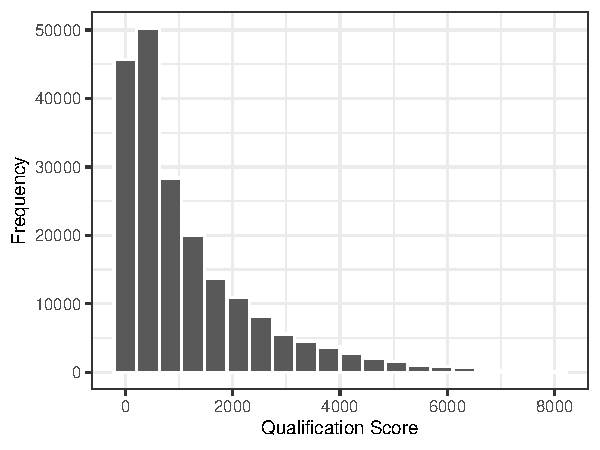
\includegraphics{draft_files/figure-latex/unnamed-chunk-3-1.pdf}
\caption{Distribution of qualification scores}
\end{figure}

Conditional probability

From our simulations, the probability of advancing given winning the
first event is 0.9951, and the probability of advancing to the final
round for an athlete, given that they were the winner of at least one
event, is 0.9947.

Table 1 shows the average score of climbers that finished in the top 8
of the qualifying round and hence advanced to the final round.

\begin{longtable}[]{@{}rr@{}}
\caption{Average score for each qualifying rank}\tabularnewline
\toprule
qual\_rank & avg\_adv\_score \\
\midrule
\endfirsthead
\toprule
qual\_rank & avg\_adv\_score \\
\midrule
\endhead
1 & 36.0187 \\
2 & 73.6111 \\
3 & 115.3954 \\
4 & 162.2263 \\
5 & 216.0041 \\
6 & 278.1649 \\
7 & 350.3272 \\
8 & 434.5932 \\
9 & 532.1383 \\
10 & 642.3298 \\
11 & 771.0376 \\
12 & 919.1239 \\
13 & 1091.2140 \\
14 & 1291.9224 \\
15 & 1536.2010 \\
16 & 1834.3433 \\
17 & 2211.7246 \\
18 & 2695.6190 \\
19 & 3399.5684 \\
20 & 4585.3123 \\
\bottomrule
\end{longtable}

\hypertarget{correlations}{%
\subsection{Correlations}\label{correlations}}

We collected data on major climbing competitions from 2018 to 2020,
including the 2020 Continental Championships of Europe, Africa, Oceania,
Pan-America; 2019 and 2018 World Championships; 2018 Asian Games; and
2018 Asian Games. We are interested in looking at the relationships
between the ranks of the individual events and the final standings, and
we computed Kendall's Tau (Kendall Rank Correlation Coefficient).

Table is a correlation matrix between the ranks for the 2018 Youth
Olympics Women's Qualification.

It is evidently clear that there is a strong and positive correlation
between the ranks of bouldering and lead climbing, and as a results, the
standings of these two events are highly correlated with the final
rankings. On the other hand, the relationship is not as strong for speed
climbing. Thus, speed climbers are facing a huge disadvantage in this
scoring system, compared to those that are specialized in the other two
concentrations.

\begin{figure}
\centering
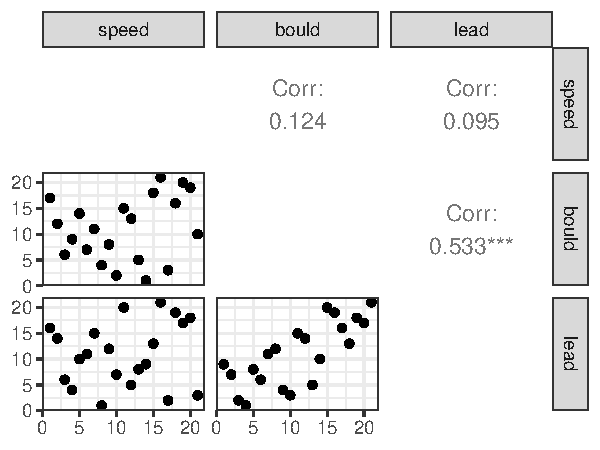
\includegraphics{draft_files/figure-latex/unnamed-chunk-7-1.pdf}
\caption{Kendall's rank correlations - 2018 World Championship, Women's
Qualification}
\end{figure}

\begin{longtable}[]{@{}lrrrr@{}}
\toprule
& rank & speed & bould & lead \\
\midrule
\endhead
rank & 1.0000000 & 0.3619048 & 0.6666667 & 0.6000000 \\
speed & 0.3619048 & 1.0000000 & 0.1238095 & 0.0952381 \\
bould & 0.6666667 & 0.1238095 & 1.0000000 & 0.5333333 \\
lead & 0.6000000 & 0.0952381 & 0.5333333 & 1.0000000 \\
\bottomrule
\end{longtable}

\end{document}
